\chapter{Mobile Instandhaltung als Anwendungskontext}
\label{chapter:kapitel3}
Beschreibung der fachlichen und technischen Rahmenbedingungen, der Instandhaltungsprozesse, 
der SAP-Fiori-Plattform sowie des konkreten Untersuchungsgegenstands.

\section{Instandhaltungsprozesse und SAP PM}
\label{section:Instandhaltungsprozesse}
Die Instandhaltung umfasst nach DIN~31051:2019-06 die Kombination aller technischen und administrativen Maßnahmen, sowie Maßnahmen des 
Managements, die während des Lebenszyklus eines Objekts dem Erhalt oder der Wiederherstellung seines funktionsfähigen Zustands 
dienen.\footcite[Vgl.][Abschnitt~3.1.1]{din31051_2019} Die Norm gliedert die Instandhaltung vollständig in vier Grundmaßnahmen: Wartung, 
Inspektion, Instandsetzung und Verbesserung.\footcite[Vgl.][Abschnitt~4]{din31051_2019} Wartung bezeichnet dabei Maßnahmen zur Verzögerung 
des Abbaus des vorhandenen Abnutzungsvorrats, die Inspektion die Prüfung der maßgeblichen Merkmale eines Objekts auf Konformität durch 
Messung, Beobachtung oder Funktionsprüfung.\footcite[Vgl.][Abschnitte~3.1.2 und~3.1.3]{din31051_2019} Die Instandsetzung ist die physische 
Wiederherstellung der Funktion eines fehlerhaften Objekts, die Verbesserung steigert Zuverlässigkeit oder Instandhaltbarkeit, ohne die 
ursprüngliche Funktion zu verändern.\footcite[Vgl.][Abschnitte~3.1.4 und~3.1.5]{din31051_2019}

Im industriellen Umfeld ist die Instandhaltung eng mit dem Erfordernis lückenloser Dokumentation verbunden. Jede der vier Grundmaßnahmen 
schließt nach der Norm Auftragsdokumentation, Durchführungsprotokoll und Rückmeldung als prozessuale Bestandteile 
ein.\footcite[Vgl.][Abschnitte~3.1.2--3.1.5]{din31051_2019} Die Dokumentation ist damit nicht allein eine administrative Anforderung, 
sondern konstitutiver Bestandteil des Instandhaltungsprozesses selbst. Im Kontext der mobilen Instandhaltung gewinnt dieser Aspekt 
besondere Bedeutung, da Techniker Maßnahmen direkt am Einsatzort erfassen und rückmelden müssen und dabei häufig ohne stationären Zugang 
zu einem PC-Arbeitsplatz arbeiten müssen.\footcite[Vgl.][S.~304-305]{eisenmann_von_2023}

Zur systemseitigen Unterstützung setzen Unternehmen \ac{ERP}-Systeme ein; im SAP-Umfeld übernimmt diese Funktion das Modul SAP~PM, das 
heute unter der Bezeichnung SAP~EAM weitergeführt wird.\footcite[Vgl.][S.~34-35]{liebstueckel_2013} SAP~PM stellt Funktionen zur 
Verwaltung technischer Objekte, insbesondere Technische Plätze und Equipments, sowie zur Planung und Abwicklung von 
Instandhaltungsmeldungen und -aufträgen bereit.\footcite[Vgl.][S.~53ff.]{liebstueckel_2013} Die Instandhaltungsmeldung ist dabei das 
zentrale Erfassungsobjekt für Störungen, Anforderungen und Befunde und bildet den Ausgangspunkt der Auftragserteilung, womit sie das 
primäre Verbindungselement zwischen Techniker und SAP-System darstellt.

\section{SAP Fiori als Designsystem und technologische Grundlage}
\label{section:fiori}

Die in Kapitel~\ref{section:Instandhaltungsprozesse} beschriebene mobile Instandhaltung wird
im untersuchten Unternehmen durch eine Anwendung unterstützt, die auf dem
Gestaltungs- und Technologierahmen von SAP Fiori beruht. Um den
Untersuchungsgegenstand (Kapitel~\ref{section:untersuchungsgegenstand}) und seine
spätere Bewertung einordnen zu können, werden im Folgenden die wesentlichen
Merkmale von SAP Fiori als Designsystem, \ac{SAPUI5} als
technologische Basis, SAP Gateway und das \ac{OData} als Integrationsschicht
sowie die Typisierung von Fiori-Anwendungen dargestellt.

Bei SAP Fiori handelt es sich um ein von SAP eingeführtes Designsystem, mit dem ein
einheitliches Erscheinungsbild und einheitliche Bedienmuster über das
SAP-Anwendungsportfolio hinweg etabliert werden
soll.\footcite[Vgl.][S.~1]{mathew_2015} Hintergrund der Entwicklung war die
Kritik an der Bedienbarkeit klassischer SAP-Oberflächen, bei denen Anwender für
einfache Vorgänge mehrere Transaktionen ausführen mussten und vertiefte
Systemkenntnisse vorausgesetzt wurden. Vor dem Hintergrund einer zunehmend von
Konsumanwendungen geprägten Erwartungshaltung rückte SAP die \ac{UX} in den
Vordergrund.\footcite[Vgl.][S.~3]{mathew_2015} Methodisch wurde Fiori auf
Grundlage des Design-Thinking-Ansatzes in Zusammenarbeit mit Kunden und Partnern
entwickelt.\footcite[Vgl.][S.~5]{szirtes_rivlin_2016} Das Designsystem ruht auf
fünf Gestaltungsprinzipien: rollenbasiert, responsiv, einfach, kohärent und
ansprechend (role-based, responsive, simple, coherent,
delightful).\footcites[Vgl.][S.~13~f.]{mathew_2015}[Vgl.][S.~5]{szirtes_rivlin_2016}
Diese Prinzipien geben einen herstellerseitig gesetzten Gestaltungsrahmen vor,
innerhalb dessen die untersuchte Anwendung entstanden ist. Sie ergänzen die in
Kapitel~\ref{grundsaetzeISO} dargestellten Interaktionsprinzipien der
ISO~9241-110, ersetzen diese jedoch nicht, da sie nicht als überprüfbarer,
normativer Bewertungsmaßstab konzipiert sind.

Technologisch basieren Fiori-Anwendungen auf SAPUI5, der von SAP bereitgestellten
Entwicklungsplattform für webbasierte
Benutzeroberflächen.\footcite[Vgl.][S.~6]{szirtes_rivlin_2016} SAPUI5 baut auf
\ac{HTML5} auf, wodurch die Oberflächen plattform- und geräteübergreifend in modernen
Browsern lauffähig sind und sich responsiv an unterschiedliche Bildschirmgrößen
anpassen.\footcite[Vgl.][S.~13]{mathew_2015} Die Oberflächen werden dabei aus produktspezifischen \ac{UI}-Komponenten
zusammengesetzt.\footcite[Vgl.][S.~20]{mathew_2015} Eine vertiefte Darstellung der
Implementierung ist für die vorliegende Arbeit nicht erforderlich. Relevant ist jedoch,
dass die untersuchte Anwendung als SAPUI5-basierte Fiori-App realisiert ist.

Die Anbindung der Oberfläche an das Backend erfolgt über SAP Gateway, das als
Middleware zwischen dem SAPUI5-Frontend und dem SAP-Backend fungiert und die
Geschäftsdaten über das \ac{OData}
bereitstellt.\footcite[Vgl.][S.~177~f.]{mathew_2015} In der typischen Architektur
transaktionaler Fiori-Anwendungen enthält der \ac{ABAP}-Frontend-Server die
Oberflächenschicht mit den SAPUI5-Komponenten sowie SAP Gateway mit dem
aktivierten OData-Service und kommuniziert über eine vertrauensbasierte Verbindung
mit dem ABAP-Backend-Server, in dem die Geschäftslogik und die Daten
liegen\footcite[Vgl.][S.~19~f.]{mathew_2015} (siehe Abbildung~\ref{abb:fiori-architektur}). Für die untersuchte Anwendung
bedeutet dies, dass die im SAPUI5-Frontend erfassten Instandhaltungsdaten über
OData-Services und SAP Gateway mit dem dahinterliegenden SAP-Backend ausgetauscht
werden.

\begin{figure}[htbp]
  \centering
  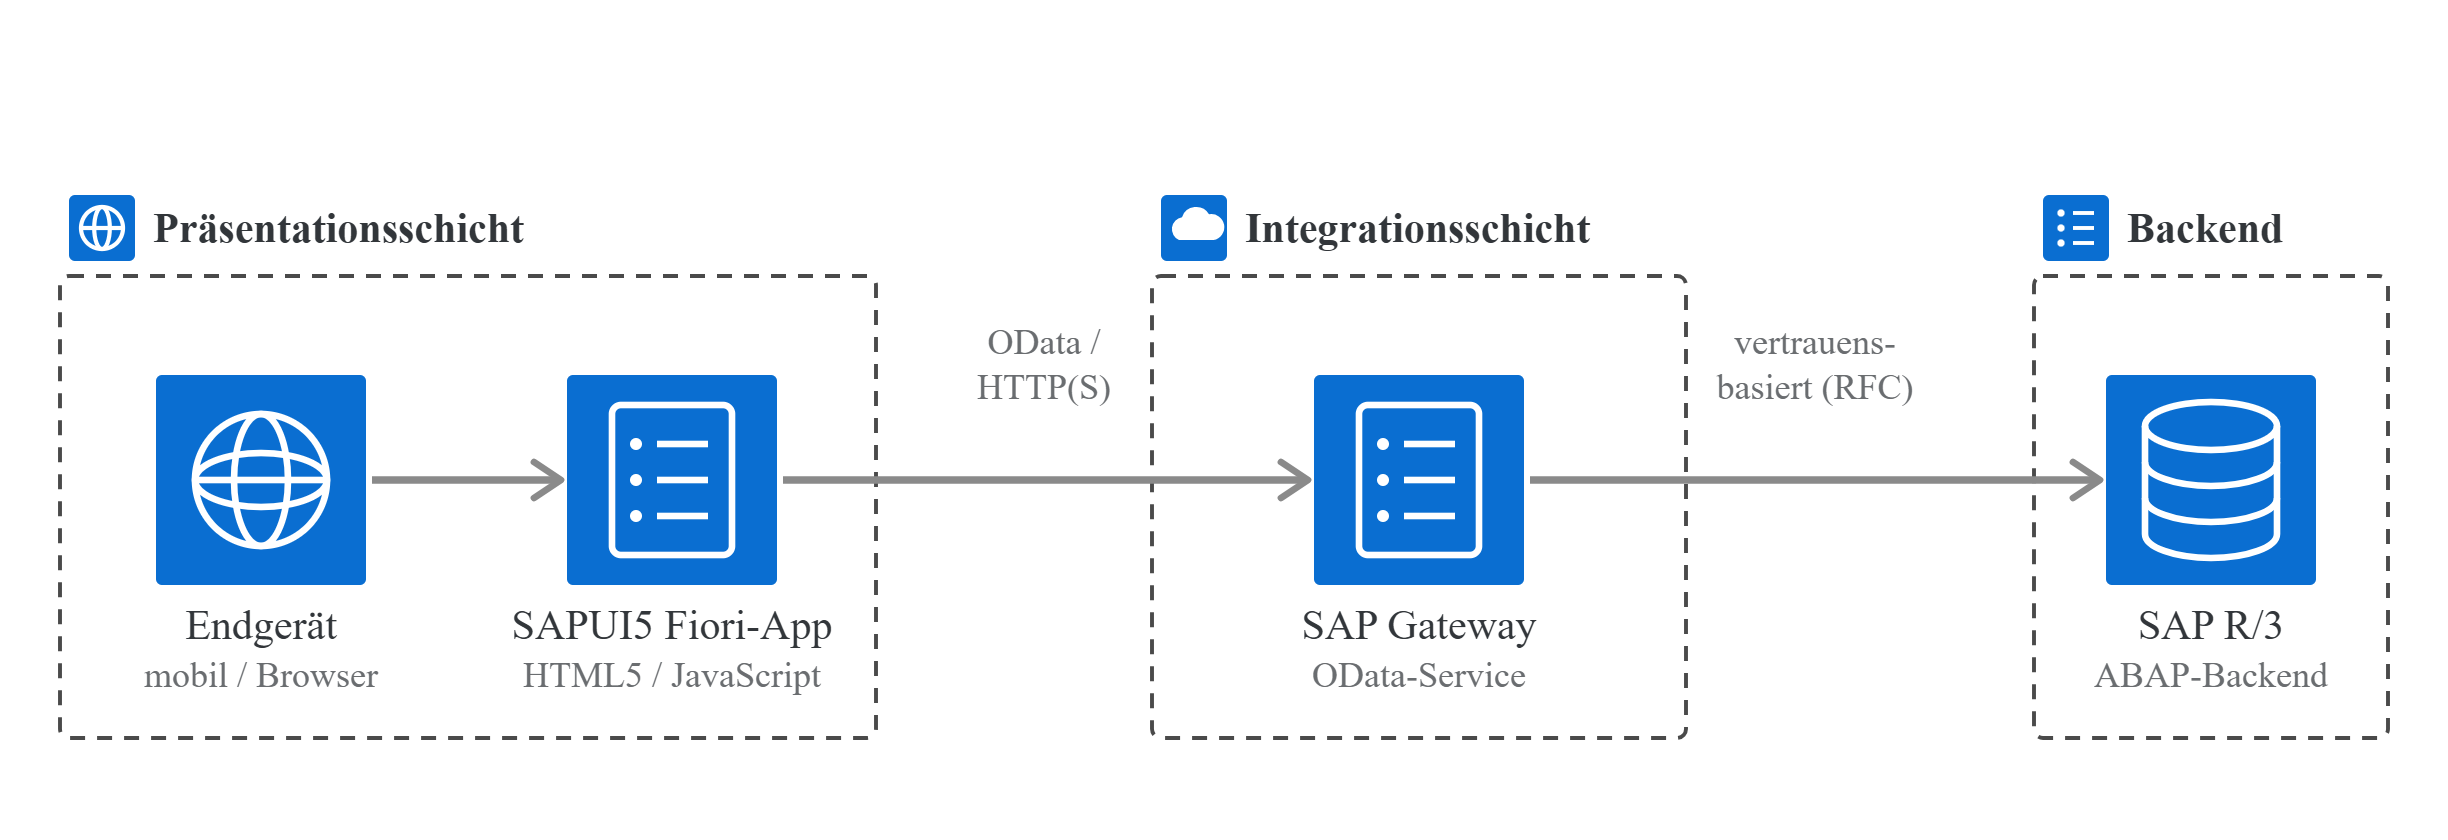
\includegraphics[width=\textwidth]{graphics/sap-fiori-architektur.png}
  \caption{Architektur einer SAPUI5-basierten Fiori-Anwendung}
  \label{abb:fiori-architektur}
\end{figure}


Neben dieser Architektur unterscheidet SAP drei Typen von Fiori-Anwendungen:
transaktionale Anwendungen, Fact-Sheet-Anwendungen und analytische
Anwendungen.\footcite[Vgl.][S.~7]{szirtes_rivlin_2016} Transaktionale Anwendungen
dienen dem aufgabenbezogenen Zugriff und ermöglichen das Ausführen von
Geschäftsvorgängen wie dem Anlegen und Bearbeiten von Belegen.\footcite[Vgl.][S.~16]{mathew_2015}
Die untersuchte Anwendung zur Dokumentation von Instandhaltungsvorgängen lässt sich
als transaktionale Fiori-Anwendung einordnen. Ihre konkrete Ausgestaltung in Form von
Funktionsumfang, Oberflächenaufbau und Nutzungskontext wird im folgenden
Kapitel~\ref{section:untersuchungsgegenstand} beschrieben.

\section{Untersuchungsgegenstand und Nutzungskontext}
\label{section:untersuchungsgegenstand}
Die im vorangegangenen Kapitel als transaktionale Anwendung eingeordnete Fiori-App »Meldung -- Foto aufnehmen« bildet den 
Untersuchungsgegenstand der vorliegenden Arbeit. Im Folgenden wird ihre konkrete Ausgestaltung beschrieben. Zunächst werden Zweck, 
Funktionsumfang, der zugrunde liegende Arbeitsablauf sowie die technische Einbettung der Anwendung dargestellt. Anschließend wird ihr 
Nutzungskontext erläutert, da die Gebrauchstauglichkeit eines interaktiven Systems stets nur in Bezug auf einen konkreten 
Verwendungszusammenhang bestimmt werden kann (vgl. Kapitel~\ref{section:usability}). Die Beschreibung von Untersuchungsgegenstand und 
Nutzungskontext bildet damit den Bewertungsrahmen für die heuristische Evaluation in Kapitel~\ref{chapter:kapitel4}.

\subsection{Untersuchungsgegenstand}

Bei der Anwendung »Meldung -- Foto aufnehmen« handelt es sich um eine SAPUI5-basierte Fiori-Anwendung, deren Aufgabe die fotografische 
Dokumentation von Instandhaltungsvorgängen ist. Ihr Zweck besteht darin, Fotos zu einer bestehenden Instandhaltungsmeldung aufzunehmen 
oder von einem Endgerät hochzuladen und diese eindeutig der jeweiligen Meldungsnummer zuzuordnen. Auf diese Weise wird eine strukturierte 
Bilddokumentation ermöglicht, die im weiteren Instandhaltungsprozess nachvollziehbar bleibt.\footnote{Vgl. Woodward L'Orange GmbH 2026, S.~5. Als firmeninterne Dokumentation wird diese Quelle nicht in den Anhang aufgenommen, kann jedoch auf Anfrage zur Begutachtung zur Verfügung gestellt werden.} Als 
Bezugsobjekt der Dokumentation dient dabei die Meldung des SAP-Moduls PM, die den zentralen Beleg zur Erfassung eines 
Instandhaltungssachverhalts bildet (vgl. Kapitel~\ref{section:Instandhaltungsprozesse}).
Der Funktionsumfang der Anwendung ist auf diesen Dokumentationszweck zugeschnitten und folgt einem festen Bearbeitungsablauf. 
Den Einstieg bildet die Auswahl einer Meldung über eine Suchhilfe, da eine freie manuelle Eingabe der Meldungsnummer nicht vorgesehen 
ist. Zur Eingrenzung des Meldungsbestands stehen Filterkriterien für Kostenstelle, Equipment, Technischer Platz, Meldungsart und 
Erstellungsdatum, sowie eine Freitextsuche über Meldungsnummer und Kurztext zur Verfügung (siehe Abb.~\ref{fig:meldungsauswahl}).\footcite[Vgl.][S.~8~ff.]{woodward2026doku}

\begin{figure}[htbp]
    \centering
    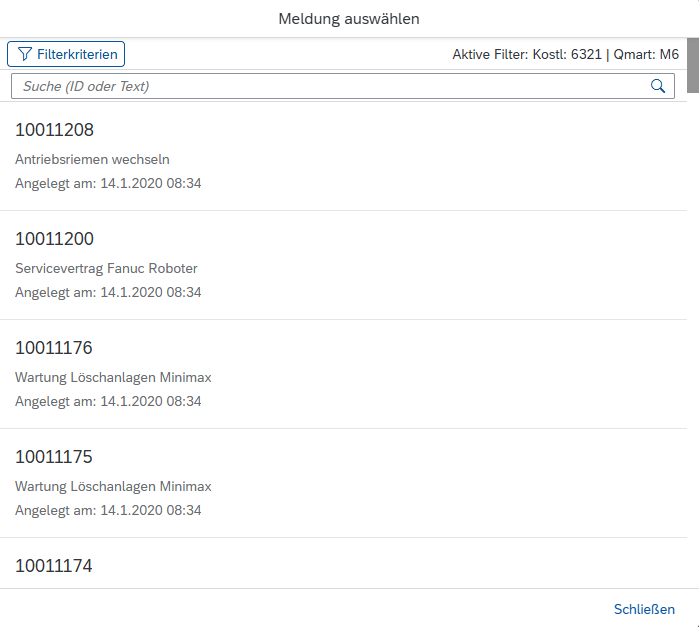
\includegraphics[width=0.7\textwidth]{graphics/meldungsauswahl.png}
    \caption{Dialog zur Meldungsauswahl in der Anwendung}
    \label{fig:meldungsauswahl}
\end{figure}

Nach Auswahl einer Meldung zeigt die Anwendung deren wesentliche Stammdaten in einem Detailbereich an, der dem Benutzer als Prüfhilfe zur 
Bestätigung der korrekten Zuordnung dient.\footcite[Vgl.][S.~15]{woodward2026doku} Erst nach Auswahl einer gültigen Meldung werden die 
Funktionen zur Fotoerfassung freigeschaltet. Dadurch wird verhindert, dass Bilder ohne Bezug zu einer Meldung erfasst 
werden (siehe Abb.~\ref{fig:hauptansicht}).\footcite[Vgl.][S.~16]{woodward2026doku}

\begin{figure}[htbp]
    \centering
    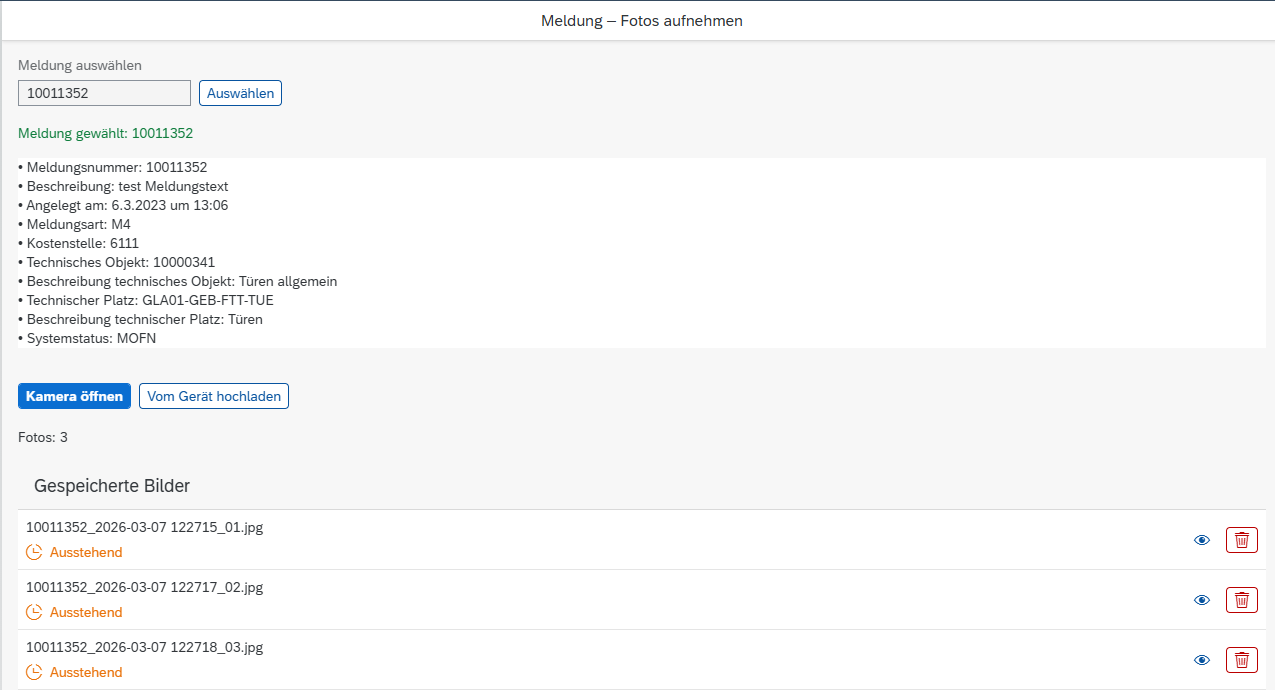
\includegraphics[width=0.7\textwidth]{graphics/hauptansicht.png}
    \caption{Hauptansicht mit Meldungsdetails und freigeschalteten Erfassungsfunktionen}
    \label{fig:hauptansicht}
\end{figure}

Die eigentliche Bilderfassung erfolgt auf zwei Wegen. Über die Gerätekamera nimmt der Benutzer ein Foto auf, das zunächst in einer 
Vorschau zur Kontrolle angezeigt und anschließend übernommen oder verworfen wird (siehe Abb.~\ref{fig:kameradialog}).  

\begin{figure}[htbp]
    \centering
    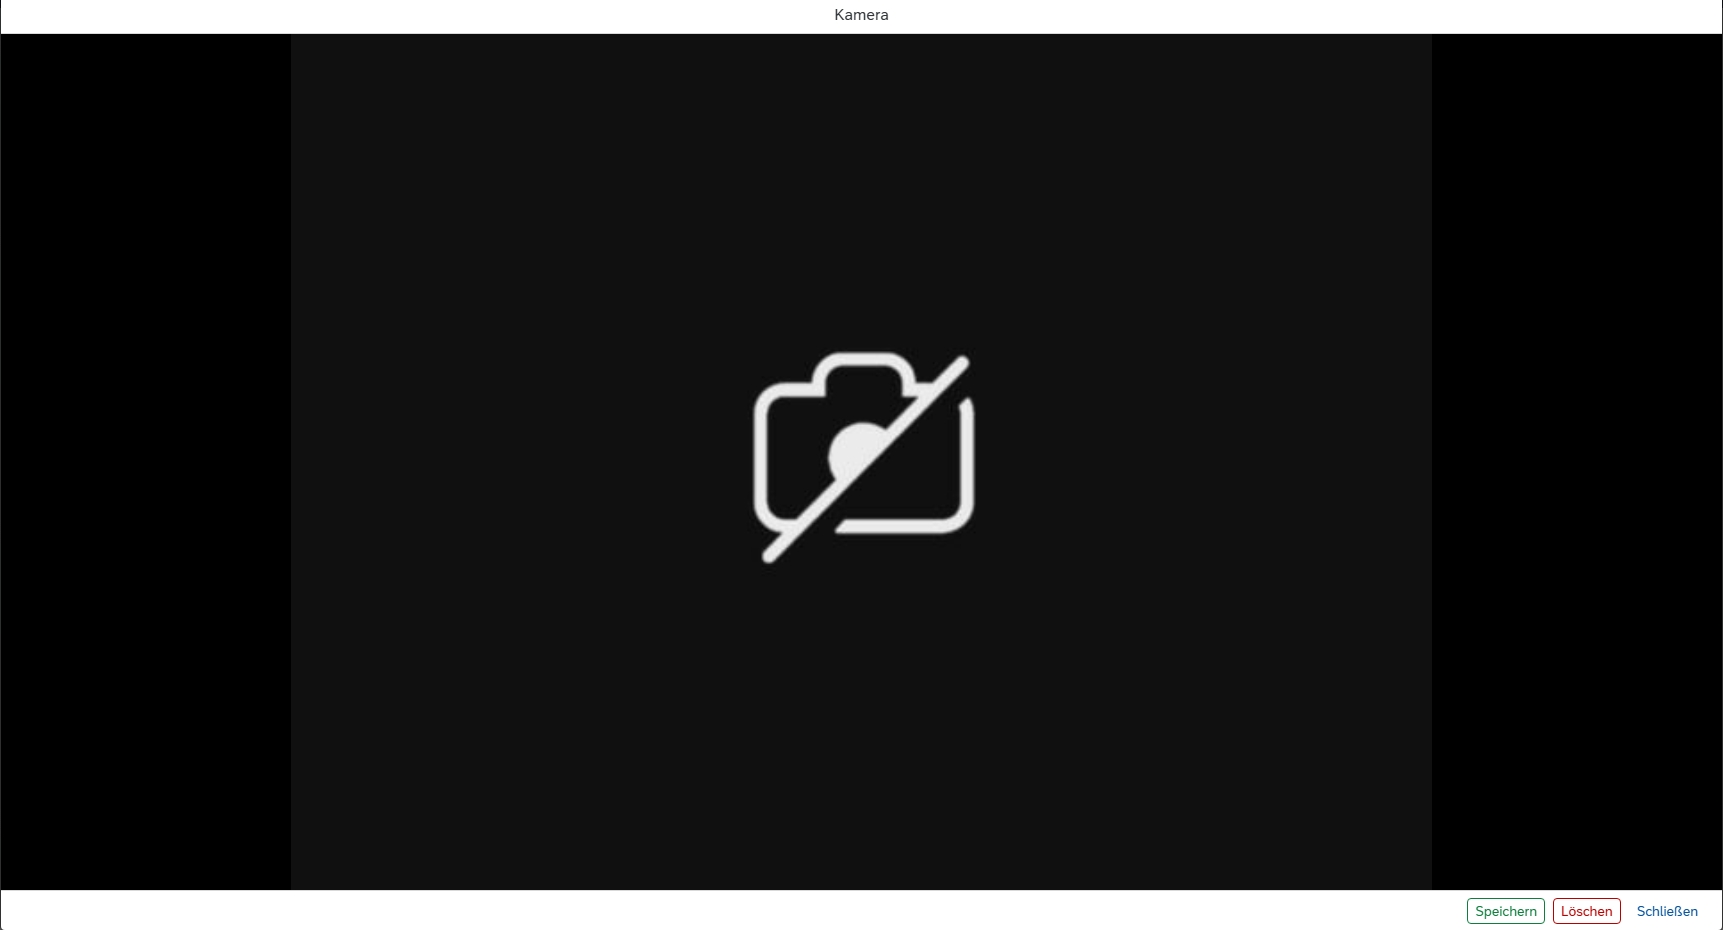
\includegraphics[width=0.7\textwidth]{graphics/kameradialog.jpeg}
    \caption{Kameradialog im Vorschau-Modus zur Kontrolle der Fotoaufnahme}
    \label{fig:kameradialog}
\end{figure}

Alternativ können bereits vorhandene Bilddateien vom 
Endgerät hochgeladen werden.\footcite[Vgl.][S.~16~ff.]{woodward2026doku} Pro Meldung ist die Erfassung auf maximal acht Fotos begrenzt. 
Die übernommenen Bilder werden in einer Fotoliste angezeigt und systematisch benannt, wobei sich der Dateiname aus der Meldungsnummer 
und einer fortlaufenden Nummer zusammensetzt.\footcite[Vgl.][S.~20~f.]{woodward2026doku}
Technologisch ist die Anwendung in die bestehende SAP-Systemlandschaft eingebettet. Die zur Meldungsauswahl benötigten Daten bezieht 
die Anwendung über OData-Services, die über das SAP Gateway bereitgestellt und an das SAP-R/3-Backend angebunden sind. Die Anwendung 
greift somit auf einen klassischen Releasestand zu und nicht auf eine S/4HANA-Umgebung.
Der Aufruf der Anwendung erfolgt browserbasiert auf dem mobilen Endgerät. Eine Besonderheit betrifft die Ablage der erfassten Bilder.
Diese werden nicht als Dokumente innerhalb des SAP-Systems gespeichert, sondern in einem je Meldung angelegten Ordner auf einem 
Fileserver abgelegt. In SAP wird lediglich ein Verweis auf diesen Ablageort hinterlegt, der in der Transaktion IW22 unter den Ablagen 
aufgerufen werden kann. Auf diese Weise bleibt die dateibasierte Bildablage fachlich an die Meldung 
gekoppelt.\footcite[Vgl.][S.~21~f.]{woodward2026doku}
Aus dieser Zweckbestimmung ergibt sich zugleich eine bewusste Abgrenzung des Funktionsumfangs. Die Anwendung dient ausschließlich der 
Fotodokumentation zu bereits bestehenden Meldungen und ermöglicht daher weder das Anlegen noch das Bearbeiten von Meldungen und verändert 
keine Meldungsdaten im SAP-System. Ihr Leistungsumfang ist damit klar auf die Erfassung, Zuordnung und Ablage von Bildern beschränkt.

\subsection{Nutzungskontext}

Die Gebrauchstauglichkeit eines interaktiven Systems lässt sich nur in Bezug auf einen konkreten Nutzungskontext beurteilen, der sich 
nach ISO 9241-11 aus den Benutzern, ihren Arbeitsaufgaben, den eingesetzten Arbeitsmitteln sowie der physischen und sozialen Umgebung 
zusammensetzt (vgl. Kapitel~\ref{section:usability}). Im Folgenden wird dieser Nutzungskontext für die untersuchte Anwendung beschrieben, 
um den Bewertungsmaßstab für die heuristische Evaluation festzulegen.
Die Anwendung richtet sich an die Mitarbeiterinnen und Mitarbeiter 
der Instandhaltung, die unmittelbar vor Ort an den Maschinen tätig sind und die App zur Dokumentation von Defekten einsetzen. Die 
Nutzergruppe umfasst etwa 20 Personen.\footnote{Vgl. Gespräch mit Kaiser 2026, Anhang~\ref{anhang:gespraech}.} 
Kennzeichnend für diese Gruppe ist, dass ihre Tätigkeit handwerklich geprägt ist und sie nur in geringem Umfang mit SAP in 
Berührung kommt. Ihr Zugriff beschränkt sich auf das Einsehen von Meldungen, während das Anlegen oder Bearbeiten von Meldungen nicht zu 
ihren Aufgaben zählt. Die in den Meldungen verwendeten SAP-spezifischen Begriffe und Schlüssel sind den Nutzenden in der Regel nicht 
geläufig.\footnote{Vgl. Gespräch mit Kaiser 2026, Anhang~\ref{anhang:gespraech}.} Die Anwendung wird in 
deutscher Sprache genutzt, eine englische Sprachfassung existiert aufgrund des US-amerikanischen Mutterkonzerns Woodward, bildet jedoch 
nicht den Gegenstand der vorliegenden Untersuchung.
Der Arbeitsumfang besteht in der fotografischen Dokumentation von Defekten, die im Rahmen der Instandhaltung festgestellt werden und 
von routinemäßigen Arbeiten abweichen. Die Fotos werden bereits während des Feststellens des Defekts aufgenommen und dienen der späteren 
Schadensanalyse. Die Nutzung der Anwendung ist nicht verbindlich vorgeschrieben, sondern liegt im Ermessen der einzelnen Mitarbeitenden.

Eingeführt wurde sie im Auftrag des Meisters der Instandhaltung.\footnote{Vgl. Gespräch mit Kaiser 2026, Anhang~\ref{anhang:gespraech}.} 
Über die gesamte Gruppe betrachtet kommt die Anwendung täglich zum Einsatz, von der einzelnen 
Person wird sie hingegen nur etwa zweimal wöchentlich verwendet. Aus dieser Nutzungsfrequenz folgt, dass die Anwendung für die einzelnen 
Nutzenden kein routinemäßig eingeübtes Werkzeug darstellt, sondern eher gelegentlich bedient wird.\footnote{Vgl. Gespräch mit Kaiser 2026, Anhang~\ref{anhang:gespraech}.}
Als Arbeitsmittel dient ein dienstliches Smartphone, auf dem die Anwendung browserbasiert aufgerufen wird. Die Datenverbindung erfolgt 
über das \ac{WLAN} des Standorts. Die Nutzung findet in der Produktionshalle unmittelbar an den Maschinen statt und ist dort durch Lärm, 
Schmutz, Ölrückstände und beengte Platzverhältnisse geprägt. Schutzausrüstung in Form von Schutzbrillen gehört zur üblichen 
Arbeitssituation und je nach Art des Defekts werden zudem zeitweise Handschuhe getragen, die die Bedienung des Touchscreens situativ 
erschweren können. Für die Dokumentation selbst steht den Mitarbeitenden ausreichend Zeit zur 
Verfügung.\footnote{Vgl. Gespräch mit Kaiser 2026, Anhang~\ref{anhang:gespraech}.}
Der beschriebene Nutzungskontext bildet den Maßstab, an dem die Gebrauchstauglichkeit der Anwendung im folgenden Kapitel zu messen ist. 
Insbesondere die Kombination aus geringer SAP-Vertrautheit der Nutzenden, der nur gelegentlichen Verwendung und den anspruchsvollen 
Umgebungsbedingungen lässt erwarten, dass an die Verständlichkeit und die Bedienbarkeit der Anwendung besondere Anforderungen zu stellen 
sind. Vor diesem Hintergrund werden die Interaktionsprinzipien der ISO 9241-110 im folgenden Kapitel zu einem Kriterienkatalog 
operationalisiert und auf die Anwendung angewendet.

